\documentclass[english]{article}

\usepackage[latin9]{inputenc}
\usepackage[letterpaper]{geometry}
\geometry{verbose,tmargin=1in,bmargin=1in,lmargin=1in,rmargin=1in}
\usepackage{amsmath}
\usepackage{amssymb}
\usepackage{graphicx}
\usepackage{float}
\usepackage{array}
\usepackage{tikz}
\usepackage{multirow}

\title{1D electromagnets for control of 2 permanent magnetics analysis}
\author{Denise Wong}

\begin{document}
\maketitle
\begin{center}
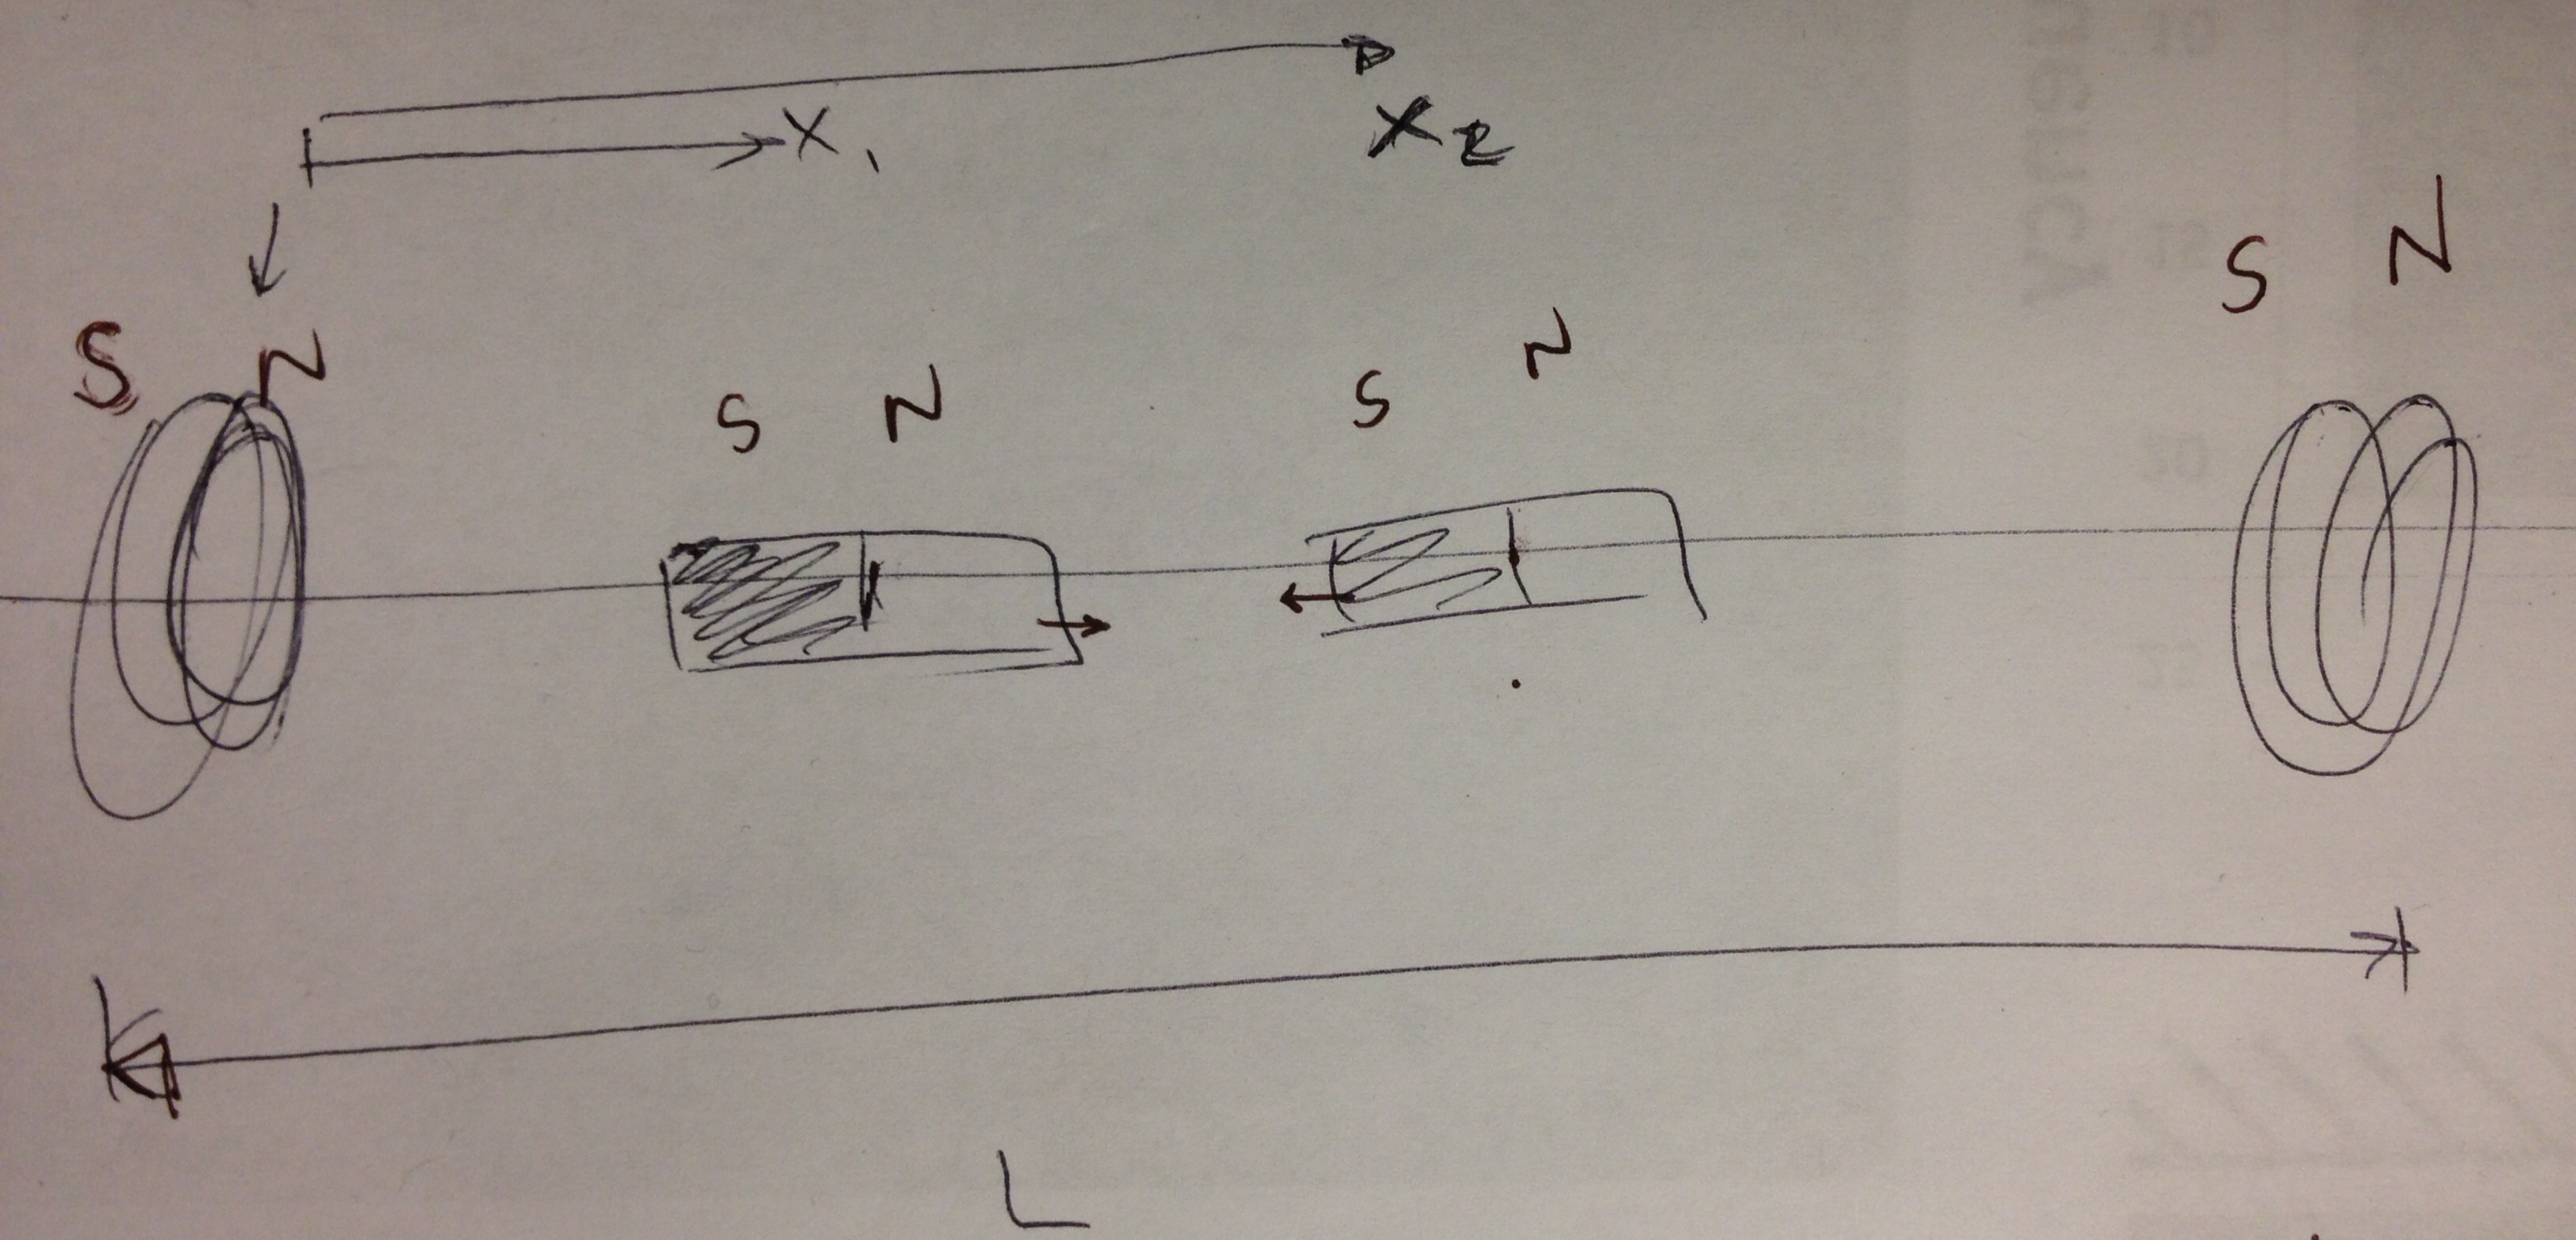
\includegraphics[width=5in]{1Dprobsetup.JPG}
\end{center}
$\mu_0$ : permeability constant $4\pi \times 10^{-7} Tm/A$\\
$\vec{\mu_j}$ : magnetic dipole moment for magnet j, $Am^2$\\
$I_i$ : current through coil i, A\\
$R_i$ : radius of coil i, m\\
$C_{perm} = \frac{\mu_0 I_p R_p^2}{2}$ : constant representing permanent magnet strength

\section*{Electromagnet}
The magnetic field on-axis of the coil is given by:
$${B}_{loop} = \frac{\mu_0 I R^2}{2\left(z^2 + R^2\right)^{3/2}}$$
${z}$ : distance from the center of the fixed electromagnet to the center of the free permanent magnet.  

\section*{Permanent Magnet}
\subsection*{Permanent Magnet modeled using classical mechanics}
Let force between 2 magnets be expressed as:
$$\vec{F} = \frac{\mu_0 m_1 m_2}{4 \pi r^2}\hat{r}$$
where $m_1,m_2$ are the magnitude of the magnetic poles of permanent magnet 1 and 2 measured in Ampere-meters (Am).  Written in the above coordinate frame for the 1D problem, the force in the x-direction acting on magnet 1:
$$F_{x,1} = \frac{\mu_0 m_1 m_2}{4 \pi \left(x_2-x_1\right)^2}$$


%\subsection*{Permanent Magnet as an electromagnet}
%Model the magnetism of the permanent magnet as a magnet field produced from currents within the magnet(e.g. permanent internal currents.)
%$${B}_{perm} = \frac{\mu_0 I R_p^2}{2\left(z^2 + R_p^2\right)^{3/2}} = C_{perm} \frac{1}{\left(z^2 + R_p^2\right)^{3/2}}$$
%
%$C_{perm} = \frac{\mu_0 I_p R_p^2}{2}$ is a constant for a permanent magnet. 
%%\section*{Force on each magnet}

\section*{Force exerted on each magnet}
Relating the magnetic field, $\vec{B}$ to the force, F:
$$F = \vec{\mu}\cdot\nabla\vec{B}$$  
For a 1D system as shown above, this simplifies to:
$$F_x = \mu\frac{d\vec{B}}{dx}$$
The force exerted on magnet 1 is given by:
$$F_{x,1} = \mu_1\left(-\frac{3 x_1 \mu_0 I_1 R_{1}^{2}}{\left(x_1^2 + R_1^2 \right)^{\frac{5}{2}}} - \frac{3 \left( x_1 - L \right) \mu_0 I_2 R_{2}^{2}}{\left(\left(x_1 - L \right)^2 + R_2^2 \right)^{\frac{5}{2}}} \right) + \frac{\mu_0 m_1 m_2}{4 \pi \left(x_2-x_1\right)^2}$$

The force exerted on magnet 2 is given by:
$$F_{x,2} = \mu_2\left(-\frac{3 x_2 \mu_0 I_1 R_{1}^{2}}{\left(x_2^2 + R_1^2 \right)^{\frac{5}{2}}} - \frac{3 \left( x_2 - L \right) \mu_0 I_2 R_{2}^{2}}{\left(\left(x_2 - L \right)^2 + R_2^2 \right)^{\frac{5}{2}}} \right) - \frac{\mu_0 m_1 m_2}{4 \pi \left(x_1-x_2\right)^2}$$

Setting the above equations so that force is 0 to find the equilibrium point and writing these 2 equations in matrix form to solve for the input current:


\begin{center}
$\begin{bmatrix}
	-\frac{\mu_0 m_1 m_2}{4\pi \left(x_2-x_1\right)^2} \\[0.3em]
	\frac{\mu_0m_1m_2}{4\pi \left(x_2-x_1\right)^2}	
\end{bmatrix}
$=$
\begin{bmatrix}
			-\mu_1\frac{3 x_1 \mu_0 R_{1}^{2}}{\left(x_1^2 + R_1^2 \right)^{\frac{5}{2}}}  & -\mu_1\frac{3 \left( x_1 - L \right) \mu_0 R_{2}^{2}}{\left(\left(x_1 - L \right)^2 + R_2^2 \right)^{\frac{5}{2}}}\\
			-\mu_2\frac{3 x_2 \mu_0 R_{1}^{2}}{\left(x_2^2 + R_1^2 \right)^{\frac{5}{2}}} & -\mu_2\frac{3 \left( x_2 - L \right) \mu_0 R_{2}^{2}}{\left(\left(x_2 - L \right)^2 + R_2^2 \right)^{\frac{5}{2}}}\\
\end{bmatrix}
\begin{bmatrix}
	I_1\\ I_2
\end{bmatrix}
$
\end{center}

By inspecting the determinant of the 2x2 matrix, it can be shown that a solution for the 2 currents through the coil exists as long as $x_1 \neq x_2$, a configuration that is not physically possible.

\section*{Potential Function}
The potential function can be used to explore the stability of a system.  It is related to the force on a system by:
$$ F = -\frac{dU}{dx}$$
Given that for magnets, $\vec{F_j} = \vec{\mu_j} \bullet \frac{d\vec{B}}{dx}$, the potential function, U, is a function of the magnetic field, B.  Assuming that $\vec{\mu}_j$ is a constant, the potential function in the x direction for the j-th permanent magnet: \\
$$ U_{x,j} = -\int_{x_i}^{x} F_x dx + U(x_i) = - \mu_{x,j}B_x$$

%%% ---------------------- %%%%
%\subsection*{Permanent magnet modeled as electromagnet}
%The magnetic field on the j-th permanent magnet:
%$$B_{x,j} = \frac{\mu_0 I_1 R_{1}^{2}}{2 \left(x_j^2 + R_1^2 \right)^{\frac{3}{2}}} + \frac{\mu_0 I_2 R_{2}^{2}}{2 \left(\left(x_j - L \right)^2 + R_2^2 \right)^{\frac{3}{2}}} + C_{perm}\frac{1}{\left(\left(x_j-x_k\right)^2  +R_p^2\right)^{\frac{3}{2}}}$$
%
%Potential function in the x-direction along the axis of the electromagnetic coils for 1st magnet:
%$$ U = \mu_1\left(\frac{\mu_0 I_1 R_{1}^{2}}{2 \left(x_1^2 + R_1^2 \right)^{\frac{3}{2}}} + \frac{\mu_0 I_2 R_{2}^{2}}{2 \left(\left(x_1 - L \right)^2 + R_2^2 \right)^{\frac{3}{2}}} + C_{perm}\frac{1}{\left(\left(x_1-x_2\right)^2  +R_p^2\right)^{\frac{3}{2}}}\right)$$
%%%% ---------------------- %%%%


\subsection*{Permanent magnet modeled using classical mechanics}
To compute the potential function component from this interaction:
$$U_{perm} = -\int_{x_i}^{x}F dx + U\left(x_i\right) = -\int_{x_i}^{x_1}\frac{\mu_0 m_1 m_2}{4 \pi \left(x_2-x_1\right)^2} dx_1 + U\left( x_i \right) = -\left[-\frac{\mu_0 m_1 m_2}{4\pi \left(x_1 - x_2\right)} \right]_{x_i}^{x_1} + U\left(x_i\right)$$
Letting $-\frac{\mu_0 m_1 m_2}{4\pi \left(x_i - x_2\right)} + U\left(x_i\right) = 0$.  

The expression for the potential function for magnet 1 in the above system is therefore:
$$U_1 = \mu_1\left(\frac{\mu_0 I_1 R_{1}^{2}}{2 \left(x_1^2 + R_1^2 \right)^{\frac{3}{2}}} + \frac{\mu_0 I_2 R_{2}^{2}}{2 \left(\left(x_1 - L \right)^2 + R_2^2 \right)^{\frac{3}{2}}} \right) + \frac{\mu_0 m_1 m_2}{4\pi \left(x_2 - x_1\right)}$$


The expression for the potential function for magnet 2 in the above system is therefore:
$$U_2 = \mu_1\left(\frac{\mu_0 I_1 R_{1}^{2}}{2 \left(x_2^2 + R_1^2 \right)^{\frac{3}{2}}} + \frac{\mu_0 I_2 R_{2}^{2}}{2 \left(\left(x_2 - L \right)^2 + R_2^2 \right)^{\frac{3}{2}}} \right) + \frac{\mu_0 m_1 m_2}{4\pi \left(x_1 - x_2\right)}$$


\section*{Stability analysis}
The Hessian matrix is computed to determine the stability of the equilibrium point, where $\frac{dU}{dx_1}=0$:

$$H = \begin{bmatrix}
	\frac{\partial ^2 U}{\partial x_1^2} & \frac{\partial ^2 U}{\partial x_1 \partial x_2}\\
	\frac{\partial ^2 U}{\partial x_2 \partial x_1} & \frac{\partial ^2 U}{\partial x_2^2}
\end{bmatrix}
$$

For magnet 1:
$$H_1 = \begin{bmatrix}
	\frac{\partial ^2 U_1}{\partial x_1^2} & \frac{\partial ^2 U_1}{\partial x_1 \partial x_2}\\
	\frac{\partial ^2 U_1}{\partial x_2 \partial x_1} & \frac{\partial ^2 U_1}{\partial x_2^2}
\end{bmatrix}
\\=
\begin{bmatrix}
	\left(\frac{-3}{\left(\left(x_1 - L\right)^2 + R_2^2\right)^{\frac{5}{2}}} + \frac{15\left(x_1-L\right)^2}{\left(\left(x_1 - L\right)^2 + R_2^2\right)^{\frac{7}{2}}} + \frac{15x_1^2}{\left(R_1^2 + x_1^2 \right)^{\frac{7}{2}}} - \frac{3}{\left(R_1^2 + x_1^2 \right)^{\frac{5}{2}}} + \frac{2}{\left(x_2-x_1\right)^3}\right)
	& 
	-\frac{2}{\left(x_2-x_1\right)^3}\\
	-\frac{2}{\left(x_2-x_1\right)^3}
	&
	\frac{2}{\left(x_2-x_1\right)^3}
\end{bmatrix}
$$

For magnet 2:
$$H_2 = \begin{bmatrix}
	\frac{\partial ^2 U_2}{\partial x_1^2} & \frac{\partial ^2 U_2}{\partial x_1 \partial x_2}\\
	\frac{\partial ^2 U_2}{\partial x_2 \partial x_1} & \frac{\partial ^2 U_2}{\partial x_2^2}
\end{bmatrix}
\\=
\begin{bmatrix}
	\frac{2}{\left(x_1-x_2\right)^3}	
	& 
	-\frac{2}{\left(x_1-x_2\right)^3}\\
	-\frac{2}{\left(x_1-x_2\right)^3}
	&
	\left(\frac{-3}{\left(\left(x_2 - L\right)^2 + R_2^2\right)^{\frac{5}{2}}} + \frac{15\left(x_2-L\right)^2}{\left(\left(x_2 - L\right)^2 + R_2^2\right)^{\frac{7}{2}}} + \frac{15x_2^2}{\left(R_1^2 + x_2^2 \right)^{\frac{7}{2}}} - \frac{3}{\left(R_1^2 + x_2^2 \right)^{\frac{5}{2}}} + \frac{2}{\left(x_1-x_2\right)^3}\right)
\end{bmatrix}
$$

Solving for the eigenvalues:


\end{document}

